\documentclass{beamer}
\usepackage{listings}
\lstset{
%language=C,
frame=single, 
breaklines=true,
columns=fullflexible
}
\usepackage{subcaption}
\usepackage{url}
\usepackage{tikz}
\usepackage{graphicx}
\usepackage{tkz-euclide} % loads  TikZ and tkz-base
%\usetkzobj{all}
\usetikzlibrary{calc,math}
\usepackage{float}
\newcommand\norm[1]{\left\lVert#1\right\rVert}
\renewcommand{\vec}[1]{\mathbf{#1}} 
\newcommand{\R}{\mathbb{R}}
\newcommand{\C}{\mathbb{C}}
\providecommand{\brak}[1]{\ensuremath{\left(#1\right)}}
\providecommand{\abs}[1]{\vert#1\vert}
\providecommand{\fourier}{\overset{\mathcal{F}}{ \rightleftharpoons}}
\providecommand{\pr}[1]{\ensuremath{\Pr\left(#1\right)}}
\providecommand{\sbrak}[1]{\ensuremath{{}\left[#1\right]}}
\usepackage[export]{adjustbox}
\usepackage[utf8]{inputenc}
\usepackage{amsmath}
\usetheme{Boadilla}
\title{Research Paper Presentation}
\author{Vijay Varma}
\institute{IITH(AI)}
\date{AI20BTECH11012}
\begin{document}
%
\begin{frame}
\titlepage
\end{frame}
\begin{frame}{Title and Authors}
%\frametitle{Prerequisites}
\begin{block}{Title}
\textbf{Assessment Study For E-Learning Using Bayesian Network}
\end{block}
\begin{block}{Authors}
\begin{itemize}
    \item Rohit B Kaliwal, CSE Dept, Visvesvaraya Technological University
    \item Dr.Santosh L Deshpande ,CSE Dept, Visvesvaraya Technological University
\end{itemize}
\end{block}
\end{frame}
\begin{frame}
\begin{block}{Abstract}
    \begin{itemize}
        \item E-Learning for educational institutions has created a challenging situation due to the COVID-19 pandemic. The universities and institutions can impart knowledge. However, evaluation of the learner’s learning and outcomes remained a challenge for them.
        \item This article aims to add its dimension towards the evaluation of outcomes especially for the learners of E-Learning platforms.
        \item To improve the learner performance of an evaluation system for classified learners, the Bayesian Network (BN) for a random process is used.
        \item This Bayesian Network was effectively implemented with the accuracy of 45\% of a slow learner, 15\% of the average learner, and 40\% of excellent learners from the required quantitative data set.
    \end{itemize}
    \end{block}
    \end{frame}
    \begin{frame}
    \begin{block}{Key Words}
       \begin{itemize}
           \item E-Learning
           \item Bayesian Network (BN)
       \end{itemize}
    \end{block}
    \end{frame}
    \begin{frame}
    \begin{block}{E-Learning}
    \begin{itemize}
        \item E-Learning, or Electronic learning, is the delivery of learning and training through digital resources.
        \item Although E-Learning is based on formalized learning, it is provided through electronic devices such as computers, tablets and even cellular phones that are connected to the internet.
        \item This makes it easy for users to learn anytime, anywhere, with very few/no restrictions.
        \end{itemize}
    \end{block}
    \end{frame}
    
    
    
    \begin{frame}
        \begin{block}{E-Learning Contd.}
            \begin{itemize}
            \item  E-Learning information is delivered to the learner which should be personalized based on the profile of the learner so that learning can be effective.
            \item E-Learning study is connected to the personalization of contented release and learner’s knowledge to measure the evolution of learner.
            \item Hence, the aim of E-Learning is not given much concentration to the assessment of the learning content.
            \item Assessment of a learner’s knowledge objective is normally done by posing a set of level of questions without documenting the learner’s capabilities.
            \item Assessment of a learner’s knowledge is a challenge in the E-Learning system.
            \end{itemize}
        \end{block}
    \end{frame}

\begin{frame}
\begin{block}{E-Learning Contd.}
\begin{itemize}

    \item Several institutes and organizations are using E-Learning since it can be more efficient than conventional education at a minor price.
    \item Just beginning E-Learning is further costly than preparing to the lecture hall resources and coaching the guide, particularly if multimedia or extremely interactive technique is used.
    \item Though, release expenses for E-Learning (contain the price of network servers and scientific support) be significantly lighter than those for lecture hall facilities, instructor time, participant journey, and work period missing to be present at lecture hall assembly. 
\end{itemize}
\end{block}
\end{frame}

    \begin{frame}
      \begin{block}{Bayesian Network (BN)}
            \begin{itemize} 
                 \item A Bayesian graph is a directed acyclic diagram within a vertex that communicates in the direction of the states along with the connections signify probabilistic associations in control.    
                 \item Bayesian Networks are a type of probabilistic graphical model that uses Bayesian inference for probability computations. 
                 \item Bayesian Networks aim to model conditional dependence, and therefore causation, by representing conditional dependence by edges in a directed graph.
                 \item Through these relationships, one can efficiently conduct inference on the random variables in the graph through the use of factors.
    \end{itemize}
    \end{block}
    \end{frame}
    \begin{frame}
    \begin{block}{Bayesian Network (BN) contd.}
       \begin{itemize}
           \item Let us define a Bayesian Network B = (A, Z) 
           \item Where, A=(W, Y), an Acyclic Directed diagram through a multiplicity of vertex connected through a position of arbitrary states $W =( W_1,\cdots, W_n)$ and Y be the edges of the diagram.
           \item  Z = \{P($W_i$ $|$ Pa($W_i$))\} is the set of probability of all vertex $W_i$ are conditional towards the state of its parents Pa($W_i$) in A.
           \item The Joint Probability Distribution of all the states $W =( W_1,\cdots, W_n)$ is 
           \begin{align}
               \pr{W_1,W_2,\cdots,W_n} = \prod \pr{W_i | Pa(W_i)} \label{eq:1}
           \end{align}
           \item In Equation \eqref{eq:1}, these techniques utilize the idea of conditional  probability, i.e., what is the probability of $W_i$ communicative to observed $W_j$.
       \end{itemize}
    \end{block}
\end{frame}
\begin{frame}
 \begin{block}{Bayesian Network (BN) Examples}
    \begin{itemize}
    \item A pattern of a straight-forward Bayesian network is given in Fig \ref{Fig-1}. Similar joint probability distribution in support of Fig \ref{Fig-1} can be printed within the outline as shown below in Equation \eqref{eq:2} using the joint probability distribution of Equation \eqref{eq:1}:
    \begin{align}
     P(I,J,K) = P(I|J,K) P(J|K) P(K) \label{eq:2}
    \end{align}
    \begin{figure}[ht]
        \centering
        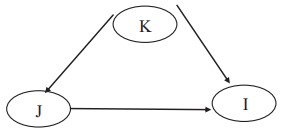
\includegraphics[width=0.5\textwidth]{Fig-1.jpg}
        \caption{Fig 1 - A Simple Bayesian Network}
        \label{Fig-1}
    \end{figure}
    \end{itemize}
 \end{block}   
\end{frame}



\begin{frame}
        \begin{figure}[ht]
            \centering
            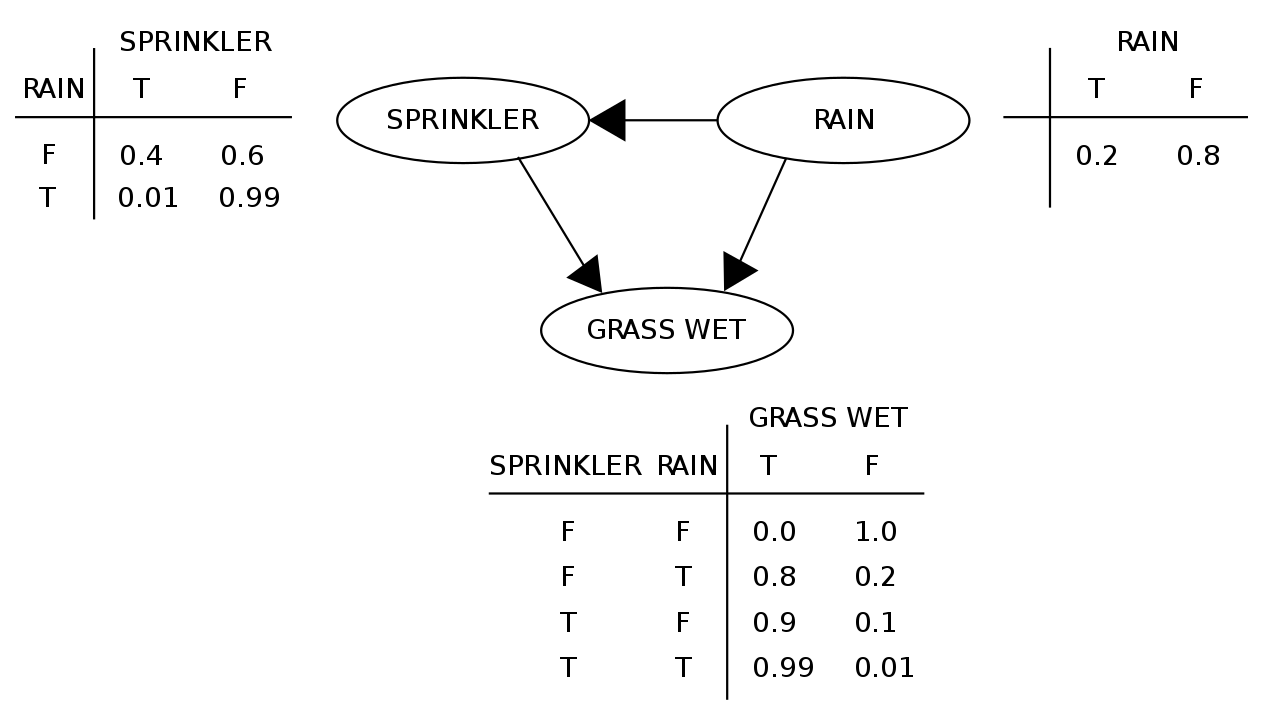
\includegraphics[width=1\textwidth]{Fig-2.png}
            \caption{Fig 2 - BN with Conditional Probability Tables (CPTs)}
            \label{Fig-2}
        \end{figure}
\end{frame}

\begin{frame}
 \begin{block}{Bayesian Network (BN) Examples}
    \begin{itemize}
    \item As in Fig \ref{Fig-2}, the two actions can root grass to be wet: a  lively sprinkler or rain. The rain has a straight result on top of the utilized sprinkler (specifically with the aim of when it rains, the sprinkler usually is not lively).
    \item These circumstances can model with a Bayesian network. Each state has 2 likely elements, T (for correct) and F (for wrong). The joint probability function is: 
    \begin{align}
     \pr{G,S,R} = \pr{G|S,R} \pr{S|R} \pr{R} \label{eq:3}
    \end{align}
    \end{itemize}
 \end{block}   
\end{frame}

\begin{frame}
 \begin{block}{Bayesian Network (BN) Examples}
    \begin{itemize}
    \item Equation \eqref{eq:3}, where G = Grass wet (correct / wrong), S = Sprinkler turned on (correct / wrong), and R = Raining (correct / wrong).
    \item "What is the probability to it is raining, known the grass is wet?" with using conditional probability formula and summing over all instances:
    \begin{align}
        \pr{R=T|G=T} &= \frac{\pr{G=T,R=T}}{\pr{G=T}} \\
        &= \frac{\Sigma_{S\in\{T,F\}}\pr{G=T,S,R=T}}{\Sigma_{S,R\in\{T,F\}}\pr{G=T,S,R}} \label{eq:5}
    \end{align}
    \item Equation \eqref{eq:5}, the extension for the joint probability function Pr (G, S, R) and the conditional probabilities as of the conditional probability tables (CPTs) known in Figure \ref{Fig-2}, single container estimate both period of the amount in the numerator and denominator.
    \end{itemize}
 \end{block}   
\end{frame}

\begin{frame}
 \begin{block}{Bayesian Network (BN) Examples}
    \begin{itemize}
    \item For example using equation \eqref{eq:3}, calculating the joint probability distribution for Pr (G, S, R) :
    \begin{multline}
        \pr{G=T,S=T,R=T} &= \pr{G=T|S=T,R=T} \\
        \pr{S=T|R=T}\pr{R=T}
    \end{multline}
    \begin{align}
        = 0.99 \times 0.01 \times 0.2 = 0.00198
    \end{align}
    \end{itemize}
 \end{block}   
\end{frame}

\begin{frame}
\begin{block}{Bayesian Network (BN) Examples}
\begin{itemize}
    \item After that the mathematical mark (sub scripted with the associated state values) is:
    \begin{multline}
        \pr{R=T|G=T}  \\
        &= \frac{0.00198_{TTT} + 0.1584_{TFT}}{0.00198_{TTT} + 0.288_{TTF} + 0.1584_{TFT} + 0.0_{TFF}} \\
        &= \frac{891}{2491} \approx 35.77\%
    \end{multline}
\end{itemize}
\end{block}
\end{frame}




\begin{frame}
\begin{block}{Implementation of E-Learning using Bayesian Networks (BN)}
\begin{itemize}
  \item The beginner knowledge assessment keen was included on an E-Learning structure to execute customized contented delivery using BN.
  \item The assessment part is executed based on track: Measured a place of stage questions for a subject individual accessible by the E-Learning framework.
  \item The position of questions is alienated into three groups such as \textbf{Satisfactory, More Satisfactory, and Most Satisfactory}.
  \item Under every position of questions, there is division. For example in the \textbf{Satisfactory Category}, built-up questions are divided into \\ 
  E = \{Much Satisfactory, More Satisfactory, Most Satisfactory\}.
  \item Likewise, questions are built-up for the last two categories such as \textbf{More Satisfactory} and \textbf{Most Satisfactory}.

\end{itemize}
\end{block}
\end{frame}

    
\begin{frame}
\begin{block}{Implementation of E-Learning using Bayesian Networks (BN) Contd.}
\begin{itemize}
    \item \textbf{A. Satisfactory Stage Questions} \\
        E1, E2, E3,$\cdots$.E27, and E30 are set of \textbf{Satisfactory Stage questions}. \\
        E1, E2, E3,$\cdots$,E9, and E30 are much satisfactory questions, \\ E10, E11, E12,$\cdots$,E18 are more satisfactory questions and \\ 
        E19, E20,$\cdots$,E22, E24,$\cdots$,E27 are most satisfactory questions.
    \item \textbf{B. More Satisfactory Stage Questions} \\
        D1, D2,……D18 and D20 are set of \textbf{More Satisfactory Stage questions}. \\
        D1, D2,….D6, and D20 are much satisfactory questions, \\
        D7, D8,….D12 are more satisfactory questions and \\ 
        D13, D14,….D18 are most satisfactory questions.
            
\end{itemize}
\end{block}
\end{frame}

\begin{frame}
\begin{block}{Implementation of E-Learning using Bayesian Networks (BN) Contd.}
\begin{itemize}
    \item \textbf{C. Most Satisfactory Stage Questions} \\
    MD1, MD2,…MD15 are set of \textbf{Most Satisfactory Stage questions}. \\
    MD1,MD2,…MD5 are much satisfactory questions, \\
    MD6,MD7,…MD10 are more satisfactory questions and \\
    MD11,MD12,…MD15 are most satisfactory questions.
    \item If E1 is False there is slightly much satisfactory question E4 than satisfactory question E1 in \textbf{Satisfactory Stage Questions} as shown in Fig \ref{Fig-3}, and if E1 is True then more satisfactory question E10 in satisfactory level questions as shown in Fig \ref{Fig-3}.
    \item If E10 is False there are slightly much satisfactory question E11 than more satisfactory question E10 in \textbf{Satisfactory Stage Questions} as shown in Fig \ref{Fig-3}, and if E10 is true then more satisfactory question E19 in \textbf{Satisfactory Stage Questions} as shown in Fig \ref{Fig-3}.
\end{itemize}
\end{block}
\end{frame}

\begin{frame}
        \begin{figure}[ht]
            \centering
            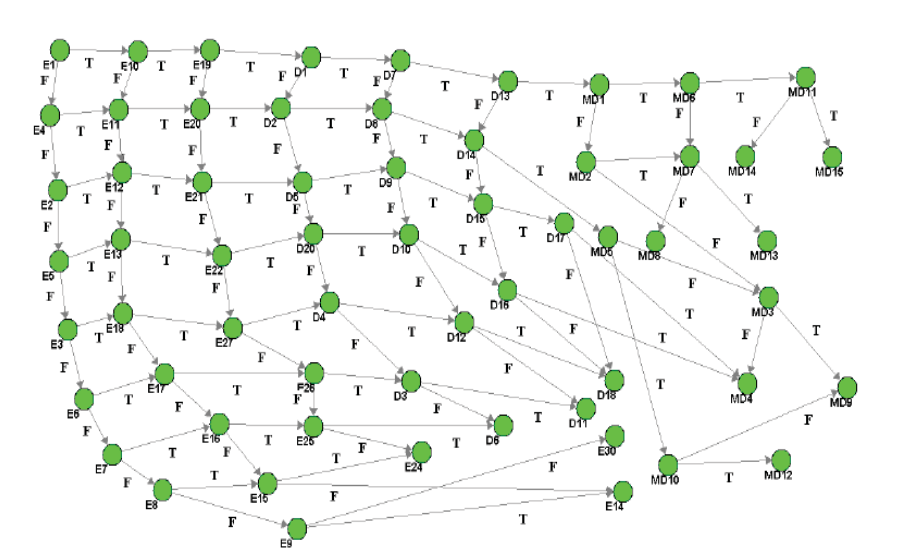
\includegraphics[width=1\textwidth]{Fig-3.png}
            \caption{Fig 3 - Learner Bayesian Network Level Questions}
            \label{Fig-3}
        \end{figure}
\end{frame}

\begin{frame}
\begin{block}{Implementation of E-Learning using Bayesian Networks (BN) Contd.}
\begin{itemize}
    \item There are nine-stage values \\
    Where, \\
    1) E1, E2, E3, E4, E5, E6, E7, E8, E9 and E30 are 1st stage. \\
    2) E10, E11, E12, E13, E14, E15, E16, E17 and E18 are 2nd stage. \\ 
    3) E19, E20, E21, E22, E24, E25, E26 and E27 are 3rd stage. \\
    4) D1, D2, D3, D4, D5, D6, and D20 are 4th stage. \\
    5) D7, D8, D9, D10, D11, and D12 are 5th stage. \\
    6) D13, D14, D15, D16, D17, and D18 are 6th stage. \\ 
    7) MD1, MD2, MD3, MD4, and MD5 are 7th stage. \\
    8) MD6, MD7, MD8, MD9, and MD10 are 8th stage. \\
    9) MD11, MD12, MD13, MD14, and MD15 are 9th stage.
\end{itemize}
\end{block}
\end{frame}

\begin{frame}
\begin{block}{Implementation of E-Learning using Bayesian Networks (BN) Contd.}
\begin{itemize}
    \item If the learner answers the 1st stage of the set of questions true then only he will be going to the next stage i.e., 2nd stage of the level of questions in the same level of \textbf{Satisfactory Stage Questions} as shown in Fig \ref{Fig-3}.
    \item If the learner answers true in all the stages in \textbf{Satisfactory Stage Questions}, then he will be going to the next level of \textbf{More Satisfactory Stage Questions}.
    \item If the learner answers the 1st stage of the set of questions false then he will be in the same stage i.e., 1st stage of the level of questions in the same level of \textbf{Satisfactory Stage Questions} as shown in Fig \ref{Fig-3}, so on for the next of the stages.
\end{itemize}
\end{block}
\end{frame}

\begin{frame}
\begin{block}{Implementation of E-Learning using Bayesian Networks (BN) Contd.}
\begin{itemize}
    \item The below Table depicts the Questions contain two potential standards Probability Correct (PC for true) and Probability Incorrect (PI for false).
     \begin{figure}[ht]
            \centering
            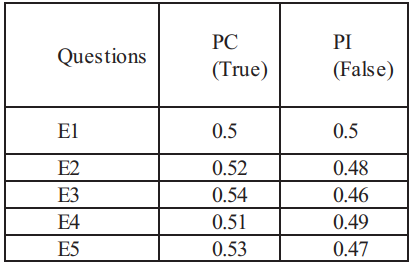
\includegraphics[width=0.7\textwidth]{Fig-4.png}
            \caption{Table I - Conditional Probabilities}
            \label{Fig-4}
        \end{figure}
\end{itemize}
\end{block}
\end{frame}

\begin{frame}
\begin{block}{Results and Discussions}
\begin{itemize}
    \item Fig \ref{Fig-5} and Fig \ref{Fig-6} shows the learner performance of learner whose outline is capture through the E-Learning framework. The content was delivered based on the learner's outline. 
    \item In Fig \ref{Fig-5} the learner has answered the different categories of levels like E1 to MD15, whereas in Fig \ref{Fig-6} the learner also answered the different categories of levels like E1 to MD13.
    \item But in Fig \ref{Fig-6} the learner has answered incorrect level in MD1, and then he/she will be at the same level as shown in Fig \ref{Fig-3} shows in the learner network.
    \item If the learner answers only the \textbf{Satisfactory Stage} of questions, then the learner is a Slow Learner, whereas the learner answers \textbf{Satisfactory Stage} and \textbf{More Satisfactory Stage} of questions, then the learner is an Average Learner.
    \item And if the learner answers \textbf{Satisfactory Stage}, \textbf{More Satisfactory Stage} and \textbf{Most Satisfactory Stage} of questions, then the learner is a Excellent Learner as shown in Fig \ref{Fig-7} based on the learner BN level of questions. 
    
\end{itemize}
\end{block}
\end{frame}


\begin{frame}
    \begin{figure}
\centering
\parbox{5cm}{
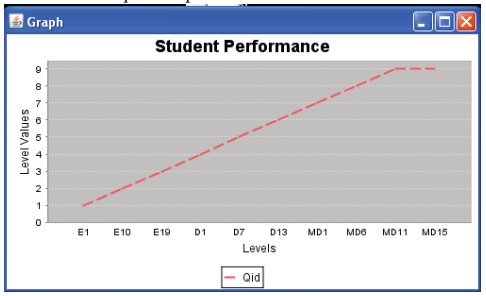
\includegraphics[width=5cm]{Fig-5.png}
\caption{Fig 5 - Learner1 Level of questions}
\label{Fig-5}}
\qquad
\begin{minipage}{5cm}
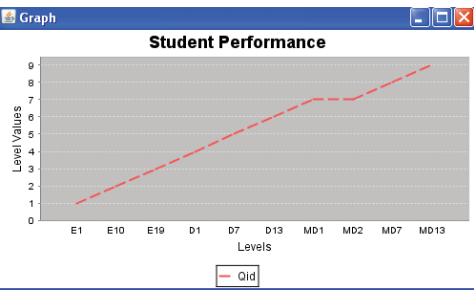
\includegraphics[width=5cm]{Fig-6.png}
\caption{Fig 6 - Learner2 Level of questions}
\label{Fig-6}
\end{minipage}
\end{figure}
\end{frame}

\begin{frame}
    \begin{figure}[ht]
            \centering
            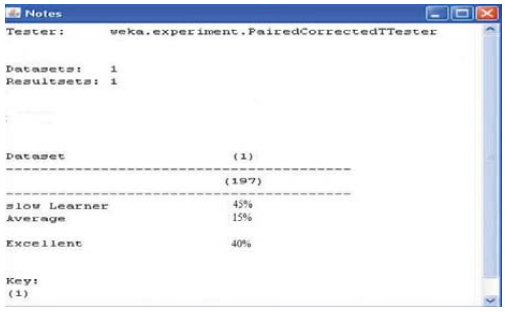
\includegraphics[width=1\textwidth]{Fig-7.png}
            \caption{Fig 7 - Learner’s Performance analysis based on BN}
            \label{Fig-7}
    \end{figure}
\end{frame}

\begin{frame}
\begin{block}{Results and Discussions Contd.}
\begin{itemize}
    \item It was observed that from Fig \ref{Fig-5} and \ref{Fig-6} that the learner performance of different levels of questions has compared between the two sets of learners to meet the learning objectives.
    \item Last but not least Fig \ref{Fig-7} shows the performance analysis based on classified learners that include slow learner, average learner, and excellent learner. By using the Learner Bayesian Network framework the result shows 45\% of a slow learner, 15\% of the average learner, and 40\% of excellent learners from the required quantitative data set.
\end{itemize}
\end{block}
\end{frame}

\begin{frame}
\begin{block}{Conclusion}
\begin{itemize}
    \item In this work, it has been implemented an assessment study for E-Learning using Bayesian Network (BN) to improve learner’s performance of an evaluation system for classified learners that include slow learner, average learner, and excellent learner.
    \item This learning is extremely helpful to recognize the percentage of a slow learner in the learners’ knowledge domain. This work is resolved the learner failures for a necessary act to upgrade the weaker learner in a complete method.
    \item Bayesian Network can provide for the execution of an additional successful E-Learning framework in the form of contented release and beginner assessment.
\end{itemize}
\end{block}
\end{frame}


\end{document}